\documentclass[10pt]{article}
\usepackage{tikz}
\usepackage[margin=0cm]{geometry}
\pagestyle{empty}

\begin{document}

\vspace*{\fill}
\begin{center}
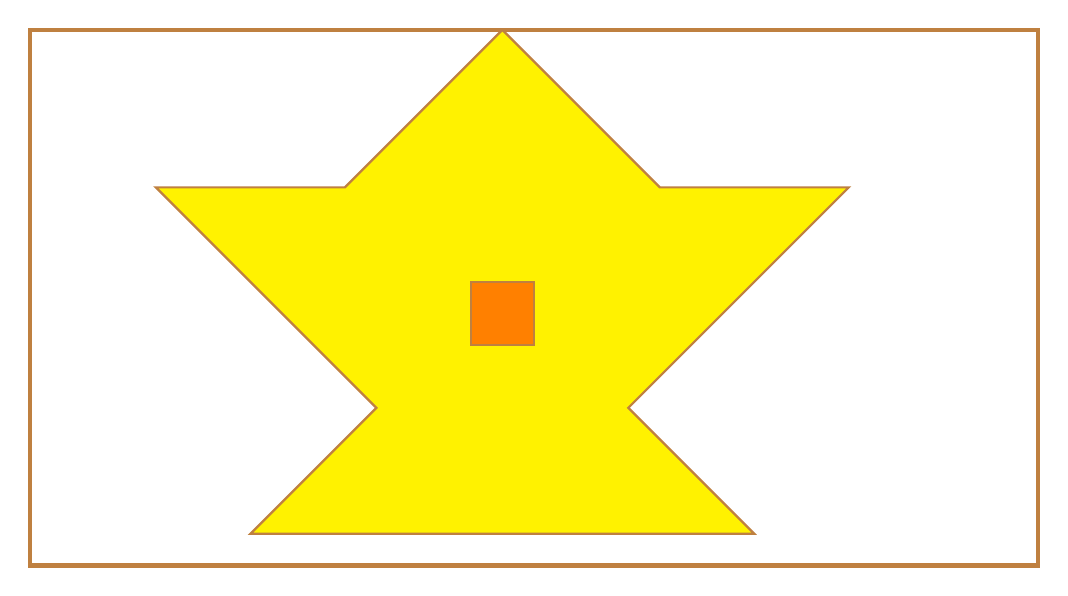
\begin{tikzpicture}[x=0.4cm, y=-0.4cm, thick, brown]
\draw[ultra thick] (0, 0) -- (32, 0) -- (32, 17) -- (0, 17) -- cycle;
%Depth 0
\filldraw[fill=orange!0!yellow] (15, 0) -- (20, 5) -- (26, 5) -- (19, 12) -- (23, 16) -- (7, 16) -- (11, 12) -- (4, 5) -- (10, 5) -- cycle;
%Depth 1
\filldraw[fill=orange!100!yellow] (14, 8) -- (16, 8) -- (16, 10) -- (14, 10) -- cycle;
\end{tikzpicture}
\end{center}
\vspace*{\fill}

\end{document}
